\documentclass[pscyr, nonums]{hedlab}
\usepackage[russian]{babel}
\usepackage[utf8]{inputenc}
\usepackage{graphicx}

\graphicspath{{images/}}

\labnum{2}
\labname{Прототипирование интерфейсов}
\student{Голубев А. В.}
\date{}

\begin{document}
    \makeheader
    \emph{Цель работы:} получение общих сведений о прототипировании интерфейсов, получение практических навыков в создании прототипов с помощью 
    ExpressionBlend \& SketchFlow.

    \emph{Задачи:}
    \begin{enumerate}\itemsep-5pt
        \item Установить ExpressionBlend \& SketchFlow
        \item Создать прототип своего сайта
    \end{enumerate}

    \begin{figure}[h!]
        \center
        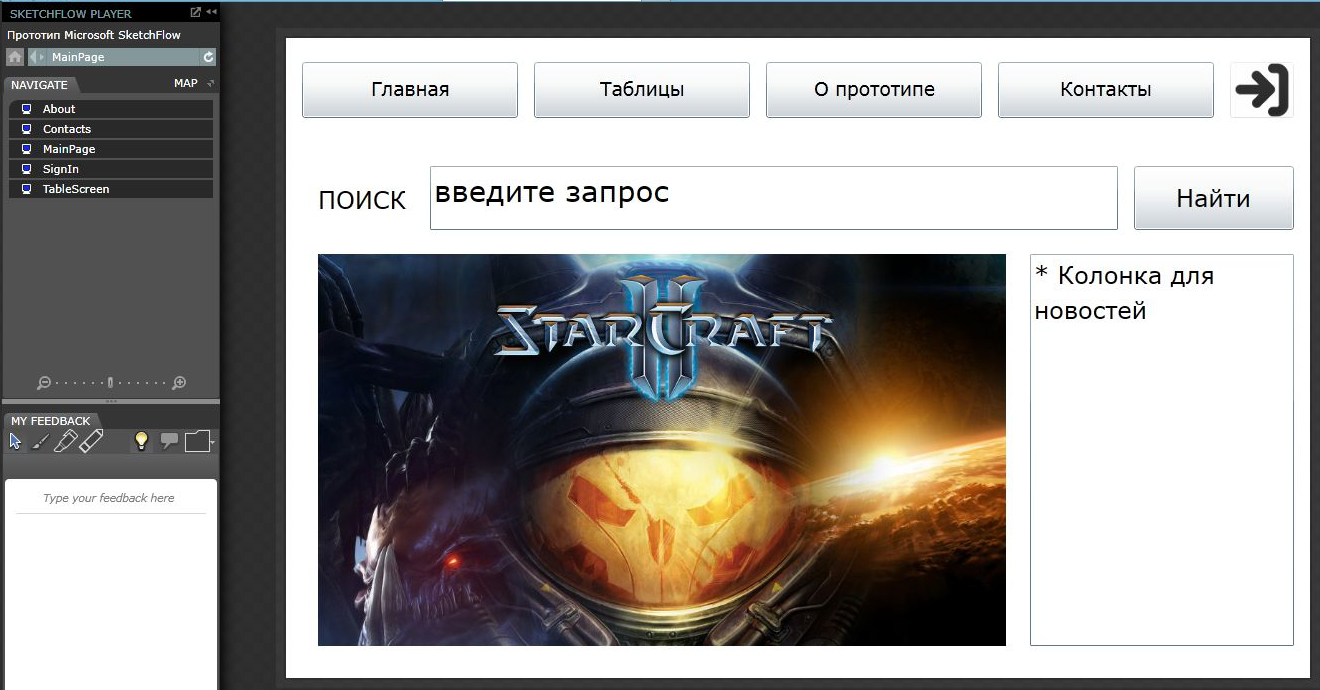
\includegraphics[width=1\textwidth]{Lab02_01}
        \caption{Прототип сайта}
    \end{figure}
\end{document}
